\documentclass[runningheads]{llncs}

\usepackage{graphicx}
\usepackage{placeins}
\usepackage{hyperref,xcolor}
\renewcommand\UrlFont{\color{blue}\rmfamily}
\usepackage{amsmath}

\begin{document}

\title{Alternatives for Neighborhood Function in Kohonen Maps \thanks{This work was supported by a private funding of Velbazhd Software LLC.}}
\titlerunning{Neighborhood in SOM}

\author{Iliyan Zankinski \and
Kolyu Kolev \and
Todor Balabanov\orcidID{0000-0003-3139-069X}}
\authorrunning{I. Zankinski et al.}

\institute{Institute of Information and Communication Technologies \\
Bulgarian Academy of Sciences \\
acad. Georgi Bonchev Str., Block 2, 1113 Sofia, Bulgaria \\
\email{iliyan@hsi.iccs.bas.bg} \\
\url{http://iict.bas.bg/}}

\maketitle

\begin{abstract}
In the field of the artificial intelligence artificial neural networks are one of the most researched topics. Multilayer perceptron has a reputation for the most used type of artificial neural network, but other types such as Kohonen maps, generalized nets\cite{tashev01} or combinations with Kalman filter\cite{alexandrov01} are also very interesting. Proposed by Teuvo Kohonen in the 1980s, self-organizing maps have application in meteorology, oceanography, project prioritization and selection, seismic facies analysis for oil and gas exploration, failure mode and effects analysis, creation of artwork and many other areas. Self-organizing maps are very useful for visualization by data dimensions reduction. Unsupervised competitive learning is used in self-organizing maps and the basic idea is the net to classify input data in predefined number of clusters. When the net has fewer nodes it achieve results similar to K-means clustering. One of the components in the self-organizing maps is the neighborhood function. It gives scaling factor for the distance between one neuron and other neurons in each step. The simplest form of a neighborhood function gives 1 for the closest nodes and 0 for all other, but the most used neighborhood function is a Gaussian function. In this research fading cosine and exponential regulated cosine functions are proposed as alternatives for neighborhood function.

\keywords{Artificial neural networks \and Self-organizing maps \and Neighborhood functions.}
\end{abstract}

\section{Introduction}

Self-organizing maps or Kohonen Neural Networks (KNNs) are networks with unsupervised training. They are very useful in finding nonlinear dependencies when data are presented in very high dimensional spaces. The projection from the high-dimensional space is usually done in a rectangular lower-dimensional space. The main idea behind KNNs is the organization of unlabeled vectors with particular features in predefined number of groups called clusters. Grid of the self-organizing map is a handy tool for convenient visualization which can reveal different features of the network. SOMs are attractive when there consist of two or more separate regions. The real goal is not to find a perfect clustering but get good idea of the cluster structure. 

\subsection{Clustering}

Clustering means a separation of the data set in set of groups. In separation where each data sample belongs exactly to only one group it is called straight clustering. If each data sample has varying degree of membership to different groups it is called fuzzy clustering.

Generally accepted concept of an optimal clustering is data set separation which minimizes the distance inside the cluster and maximizes the distance between the clusters. The most used form of distance measurement is the Euclidean norm. 

\subsection{SOM Training}

The network consists of a grid (usually two dimensional) with units. The units are connected to adjacent units with a neighborhood relation. The amount of grid units, which usually varies from a few dozen up to several thousand, gives the accuracy and generalization possibilities of the KNN. The network forms an elastic mesh that folds
as a cloud formed by the input data during training phase. Data samples lying near each other in the input space are mapped into nearby grid units. 

The network training is done iteratively. A data sample vector is randomly chosen from the input data set, as first step. As second step, distances between the selected vector and all the prototype vectors are computed. The best matching unit is the grid unit with prototype closest the selected vector. In the third step, the prototype vectors in the grid are updated. The best matching unit and its topological neighbors are moved closer to the input vector in the input space \cite{vesanto01}.

\section{Neighborhood Function}

The most used KNN's neighborhood function is the Gaussian function. In this research two alternative functions are proposed. The first function is fading cosine, which is shown in Fig.\ref{fig01}-Left. The second function is exponential regulated cosine, which is shown in FIg.\ref{fig01}-Right.

\begin{figure}
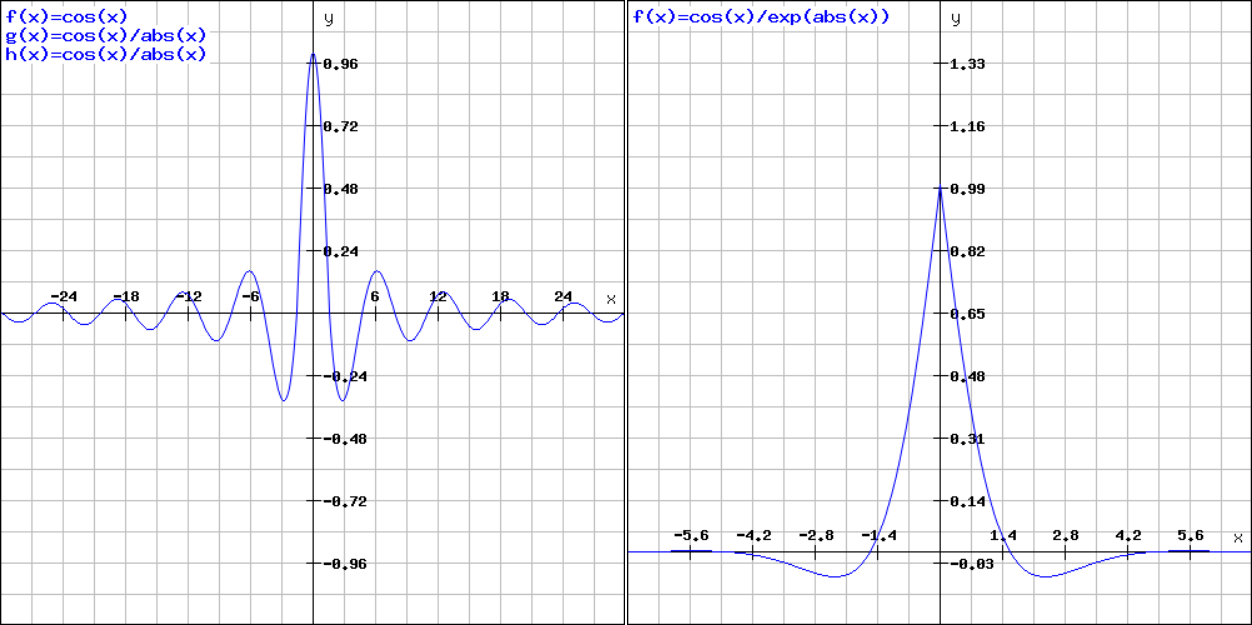
\includegraphics[width=1.0\textwidth]{fig01.png}
\centering
\caption{Left - Fading cosine neighborhood function. Right - Exponential regulated cosine neighborhood function.} \label{fig01}
\end{figure}
\FloatBarrier

The idea for the both functions is to stress grid nodes down and up. The exponential regulated cosine Eq.\ref{equ02} gives smoother stress than the fading cosine Eq.\ref{equ01}. 

\begin{equation} \label{equ01}
f(x) = 
	\begin{cases} 
		cos(x) & +\pi/2 \geq x \leq -\pi/2 \\
		\frac{cos(x)}{|x|} & -\pi/2 < x < \pi/2 \\
	\end{cases}
\end{equation}

\begin{equation} \label{equ02}
f(x) = \frac{cos(x)}{e^{|x|}}
\end{equation}

\section{Experiments and Results}

All experiments were done on a single processor desktop machine - Intel Core i5, 2.3 GHz, 2 Cores, 8GB RAM and Mac OS X 10.13.6, Apple LLVM version 9.1.0.

\section{Conclusions}

\begin{thebibliography}{8}
\bibitem{tashev01}
Tashev, T., Hristov, H.: Modeling of synthesis of information processes with generalized nets. Cybernetics and Information Technologies, \textbf{3}(2), 92--104 (2003) 
\bibitem{alexandrov01}
Alexandrov, A.: AD HOC Kalman filter based fusion algorithm for real-time Wireless Sensor Data Integration. In: FQAS-2015 Proceedings, pp. 151--160. Springer, Heidelberg (2015)
\bibitem{vesanto01}
Vesanto, J., Alhoniemi, E.: Clustering of the Self-Organizing Map. IEEE Transactions on Neural Networks, \textbf{11}(3), 586--600 (2000) 
\bibitem{angelova01}
Angelova, V.: Investigations in the Area of Soft Computing Targeted State of the Art Report. Cybernetics and Information Technologies \textbf{9}(1), 18--24 (2009)
\bibitem{atanasova01}
Atanasova T., Barova M.: Exploratory analysis of Time Series for hypothesize feature values. In: UniTech17 Proceedings,  \textbf{16}(2), 399--403 (2017)
\end{thebibliography}
\end{document}
